\documentclass[12pt, letterpaper]{report}
\usepackage[utf8]{inputenc}
\usepackage{graphicx}
\usepackage{indentfirst}
\usepackage{url}
\usepackage{titling}
\usepackage{emptypage}

\usepackage{fancyhdr}
\usepackage{acro}
\usepackage{lscape}

\graphicspath{{./images/}}

% ----- Capa -----
\newcommand{\subtitle}[1]{%
  \posttitle{%
    \par\end{center}
    \begin{center}\LARGE#1\end{center}
    \vskip0.5em}%
}

\title{\textbf{Smart City}}

\subtitle{{\large Master in Industrial Eletronics and Computers Engineering} \\ {\large Embedded Systems}}

\author{Authors:\\Diogo Fernandes PG47150\\José Tomás Abreu PG47386\\ \\ Supervisors:\\Prof. Dr. Tiago Gomes\\Prof. Ricardo Roriz\\Prof. Sérgio Pereira}

\date{\today}

%HEADER AND FOOTER CHAPTER PAGES
\fancypagestyle{plain}{%
	\fancyhf{}			%clear header and footer
	%footer
	\fancyfoot[R]{\small{\thepage}}
	\fancyfoot[L]{\small{Embedded Systems - Smart City}}
	\renewcommand{\headrulewidth}{0pt}% Line at the header invisible
	\renewcommand{\footrulewidth}{0.5pt}% Line at the footer visible
}

%HEADER AND FOOTER NORMAL PAGES
\fancypagestyle{IHA-fancy-style}{%
	%header
	\renewcommand{\headrulewidth}{0.5pt}
	\chead{\nouppercase\leftmark}
	
	%footer
	\renewcommand{\footrulewidth}{0.5pt}
	\fancyfoot[R]{\small{\thepage}}
	\fancyfoot[L]{\small{Embedded Systems - Smart City}}
	%\rfoot{\small\thepage}
	%\lfoot{\small Embedded Systems - Smart City}
}

\pagestyle{fancy}	
\fancyhf{}			%clear header and footer

\DeclareAcronym{led}{
  short=LED,
  long=Light-Emitting Diode,
}
\DeclareAcronym{iot}{
  short=IoT,
  long=Internet of Things,
}
\DeclareAcronym{hps}{
  short=HPS,
  long=High Pressure Sodium,
}
\DeclareAcronym{api}{
  short=API,
  long=Application Programming Interface,
}
\DeclareAcronym{cps}{
  short=CPS,
  long=Cyber-Physical System,
}
\DeclareAcronym{rtos}{
  short=RTOS,
  long=Real-Time Operating System,
}
\DeclareAcronym{pir}{
  short=PIR,
  long=Passive Infrared,
}
\DeclareAcronym{gpio}{
  short=GPIO,
  long=General Purpose Input/ Output,
}
\DeclareAcronym{csi}{
  short=CSI,
  long=Camera Serial Interface,
}
\DeclareAcronym{pwm}{
  short=PWM,
  long=Pulse Width Modulation,
}
\DeclareAcronym{ai}{
  short=AI,
  long=Artificial Intelligence,
}
\DeclareAcronym{gui}{
  short=GUI,
  long=Graphical User Interface,
}
\DeclareAcronym{cagr}{
  short=CAGR,
  long=Compound Annual Growth Rate,
}
\DeclareAcronym{gps}{
  short=GPS,
  long=Global Positioning System,
}
\DeclareAcronym{ldr}{
  short=LDR,
  long=Light Dependant Resistor,
}
\DeclareAcronym{ieee}{
	short=IEEE,
	long=Institute of Electrical and Electronics Engineers,
}
\DeclareAcronym{rf}{
	short=RF,
	long=Radio Frequency,
}
\DeclareAcronym{lpwan}{
	short=LPWAN,
	long=Low Power Wide Area Network,
}
\DeclareAcronym{lpwa}{
	short=LPWA,
	long=Low Power Wide Area,
}

\DeclareAcronym{nb-iot}{
	short=NB-IoT,
	long=Narrow-Band IoT,
}

\DeclareAcronym{lte-m}{
	short=LTE-M,
	long=Long Term Evolution for Machines,
}
\DeclareAcronym{unb}{
	short=UNB,
	long=Ultra-Narrow Band,
}
\DeclareAcronym{ism}{
	short=ISM,
	long=Industrial Scientific and Medical ,
}

 % load all acronyms

\begin{document}

{\begin{figure}[t]
	\centering
	
\includegraphics[width=0.35\textwidth]{EEUMLOGO}
\end{figure}}

\maketitle

%doesnt work
\cleardoublepage
\pagestyle{empty}

\pagenumbering{roman}	%roman numbering
\tableofcontents
\clearpage

\clearpage
\addcontentsline{toc}{section}{\listfigurename}\listoffigures

%\clearpage
%\addcontentsline{toc}{section}{\listtablename}\listoftables

\clearpage
\addcontentsline{toc}{section}{Acronyms}
\printacronyms

\newpage

\pagenumbering{arabic} %arabic numbering

% ---------- INTRODUCTION ----------
\pagestyle{IHA-fancy-style}
\chapter{Introduction}
% Problem statement
% Problem statement analysis
\section{Problem Statement}
Nowadays, the energy crisis is a constant theme because of the inflated energy prices \cite{energy_crisis}. Furthermore, huge energy consumption is a burden to the environment, as not all means of energy production are non-polluting. According to "Our World in Data"\cite{owidenergy}, in 2019, 63,3 \% of eletrical energy production comes from fossil fuels. It is known that, in cities, street lamps are continuously switched on at night, most of the time unnecessarily glowing with its full intensity, in the absence of any activities in the street, leading to a great waste of energy. Furthermore, it is in cities where the consequences of using cars are most noticeable. An example of this is the search for a parking space. According to the RAC Foundation \cite{cars_parked}, in England, an average car is parked 95 \% of the time, which explains how hard it can get sometimes when trying to find a parking spot. This struggle leads to an increase in carbon dioxide production as well as fuel and energy consumption.
With that in mind, the main objective of this project is the creation of a  distributed system, composed by smart street lights capable of turning on only when they detect movement in the surroundings, at night time, and also, capable of detecting available parking spaces in the street post vicinity.

\section{Problem Statement Analysis}
The main purpose of this system is to control a street lamppost, using Raspberry Pi 4B. When there is no activity in the area, the lamppost is at a predefined minimum light level, whereas when a car or pedestrian is noticed in the area, the light automatically activates. Therefore, each street lamp post  communicates wirelessly with the neighbor lamp posts, allowing to dynamically turn on the lights of the following poles. To detect movement in the vicinity of the pole, a motion detector is used, which only works during the night time. To ensure this, a luminosity sensor is used, determining the ambient light conditions. In order to facilitate the maintenance of the pole, a system that determines the operating conditions of the lamp is also implemented. When this system verifies that the lamp is not in good working conditions, that is, that it is broken or burnt, this information is transmitted to the entity responsible for the network of lampposts through a mobile app. This is also used by the person in charge, to manage all information on the pole network, such as the location and working conditions of each pole. In order to detect empty parking spots, this system should only be used in an area where there are parking spaces nearby. For this, the lamppost has a camera, turned on all day, and, after Raspberry Pi processes the acquired information, it will be available on a website, so that a user can know where parking spaces are empty.

% ---------- MARKET RESEARCH ----------
\chapter{Market Research}
% Market Research
\section{Market Definition}
Smart cities have the potential to benefit communities and individuals in a variety of applications across health, transportation, education, government, energy, and power and water. Implemented correctly, smart city applications can reduce costs, simplify services and offer a sustainable solution. \cite{smart_city_application_needs} 

\begin{figure}[ht]
	\centering
	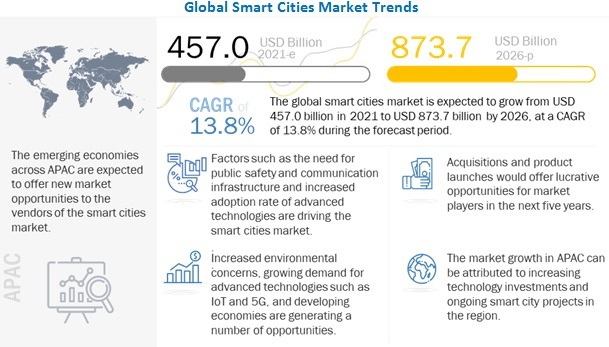
\includegraphics[width=.85\textwidth]{/02market_research/smart_cities_market}
	\caption{Global smart cities market trends.}
	\label{fig:smart_city_growth}
\end{figure}

\clearpage

As one can see, in figure \ref{fig:smart_city_growth}, according to MarketsandMarkets \cite{smart_cities_market} global smart cities market is expected to grow from USD 457 billion in 2021 to USD 873.7 billion by 2026, at a \ac{cagr} of 13.8\%, during the forecast period. Growing urbanization, need for efficient management and utilization of resources, and also the increasing demand for a healthy environment with efficient energy consumption are expected to be the major factors driving the growth of the smart cities market.

As figure \ref{fig:smart_cities_sols} shows, there are various applications of \ac{iot} technology for smart cities. In this project it will be created a solution that comprises Smart Lighting management and Smart Parking.

\begin{figure}[ht]
	\centering
	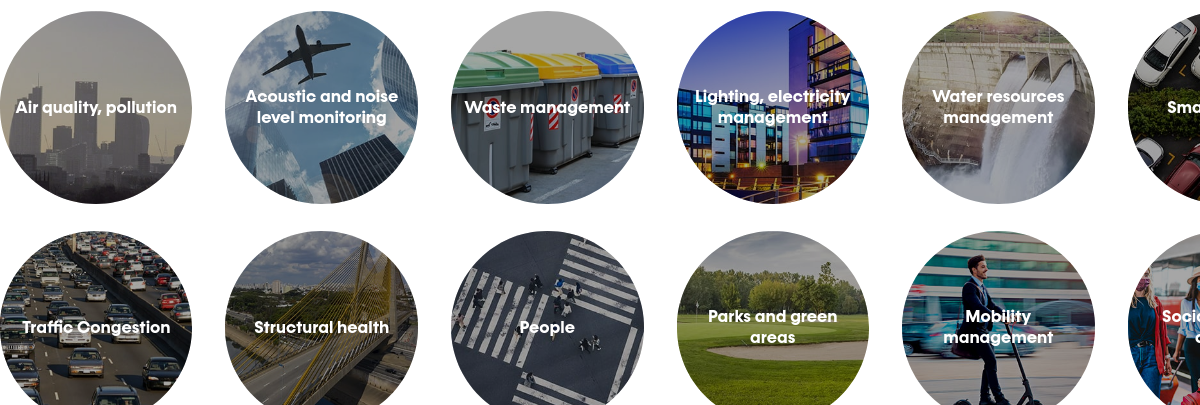
\includegraphics[width=1\textwidth]{/02market_research/applications_for_smart_cities}
	\caption{Applications of \ac{iot} technology for Smart Cities. \cite{smart_cities_solutions}}
	\label{fig:smart_cities_sols}
\end{figure}

\subsection{Smart Lighting}
Smart Street lighting is a rapidly growing lighting market, with an expected \ac{cagr} of 20.4 \% until 2026 \cite{smart_light_market}, implementing a smart management of public lighting to optimize energy consumption according to lighting needs. This is boosted by regulatory policies that encourage energy efficiency, \ac{iot} convergence and the drop of \ac{led} prices. This new concept of smart light post is also growing, implementing not only the smart management of street lights, but also features that go from basic \ac{led} replacement control, to traffic and video monitoring, environmental monitoring, and others.

\subsubsection{Telensa - PLANet}
Nowadays, Telensa is the market share leader in smart street lighting with more than ten years of experience.\cite{telensa} PLANet is an intelligent street lighting system, consisting of wireless nodes connecting individual lights, a dedicated network owned by the city and a central management application, seen in figure \ref{fig:telensa}. This system reduces energy and maintenance costs associated with street lighting and also improves quality of maintenance through automatic fault reporting.

\begin{figure}[ht]
	\centering
	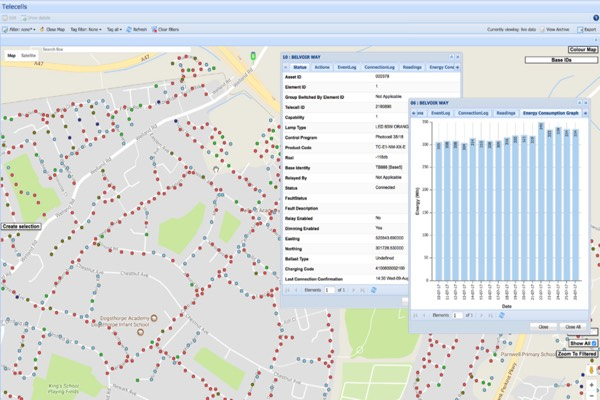
\includegraphics[width=0.8\textwidth]{/02market_research/telensa}
	\caption{Telecells - PLANet's Central Management System.}
	\label{fig:telensa}
\end{figure}

\subsubsection{FLASHNET - inteliLIGHT}
FLASHNET is a company focused on developing intelligent systems for smarter cities and better infrastructures and have created a solution that provides the right amount of light where and when needed to lighten the streets, the inteliLIGHT \cite{inteli_light}.

Using the existing infrastructure, this solution saves money and transforms the existing distribution level network into an intelligent infrastructure of the future, as shown in figure \ref{fig:intelilight}. Furthermore, the system is integrated with major \ac{iot} platforms and provides \ac{api} connectivity with City Management applications, ensuring compatibility with existing smart lighting and smart city initiatives.

\begin{figure}[ht]
	\centering
	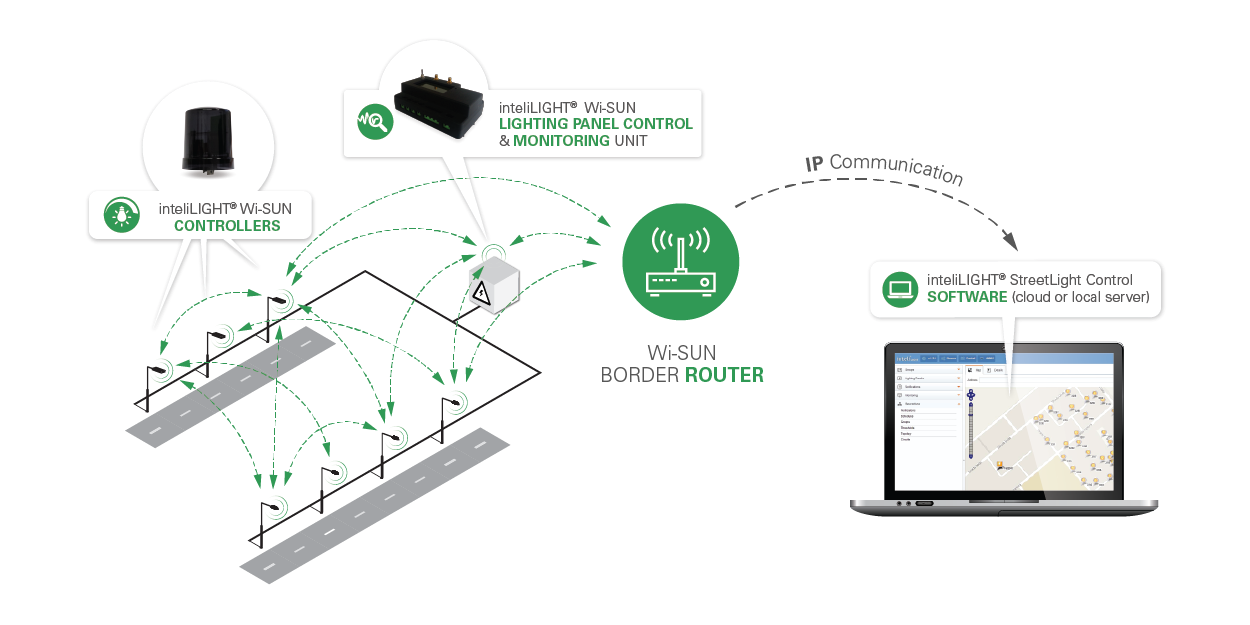
\includegraphics[width=0.95\textwidth]{/02market_research/intelilight}
	\caption{inteliLIGHT Communication Technology.}
	\label{fig:intelilight}
\end{figure}

\subsection{Smart Parking}
Smart parking, through the monitoring of parking spaces availability in the city, is also a growing market, expected to grow with a \ac{cagr} of 17.85\% in the forecast period of 2021 to 2028.\cite{smart_parking_market} The rise in investment in building driverless vehicles and an increase in the government’s initiative in building smart cities across the globe, along with the demand and adoption of \ac{iot} technology, are the main driving factors for the growth of smart parking market.

\subsubsection{intuVision - intuVision VA Parking}
Regarding only to the detection of available parking spaces, there is a solution, by intuVision, named intuVision VA Parking, which provides parking lot analytics to determine vehicle count and security, and monitor parking space availability at all times, both for cities and for private parking lots, as one can see in the figure \ref{fig:intuvision}.\cite{parking}

\begin{figure}[ht]
	\centering
	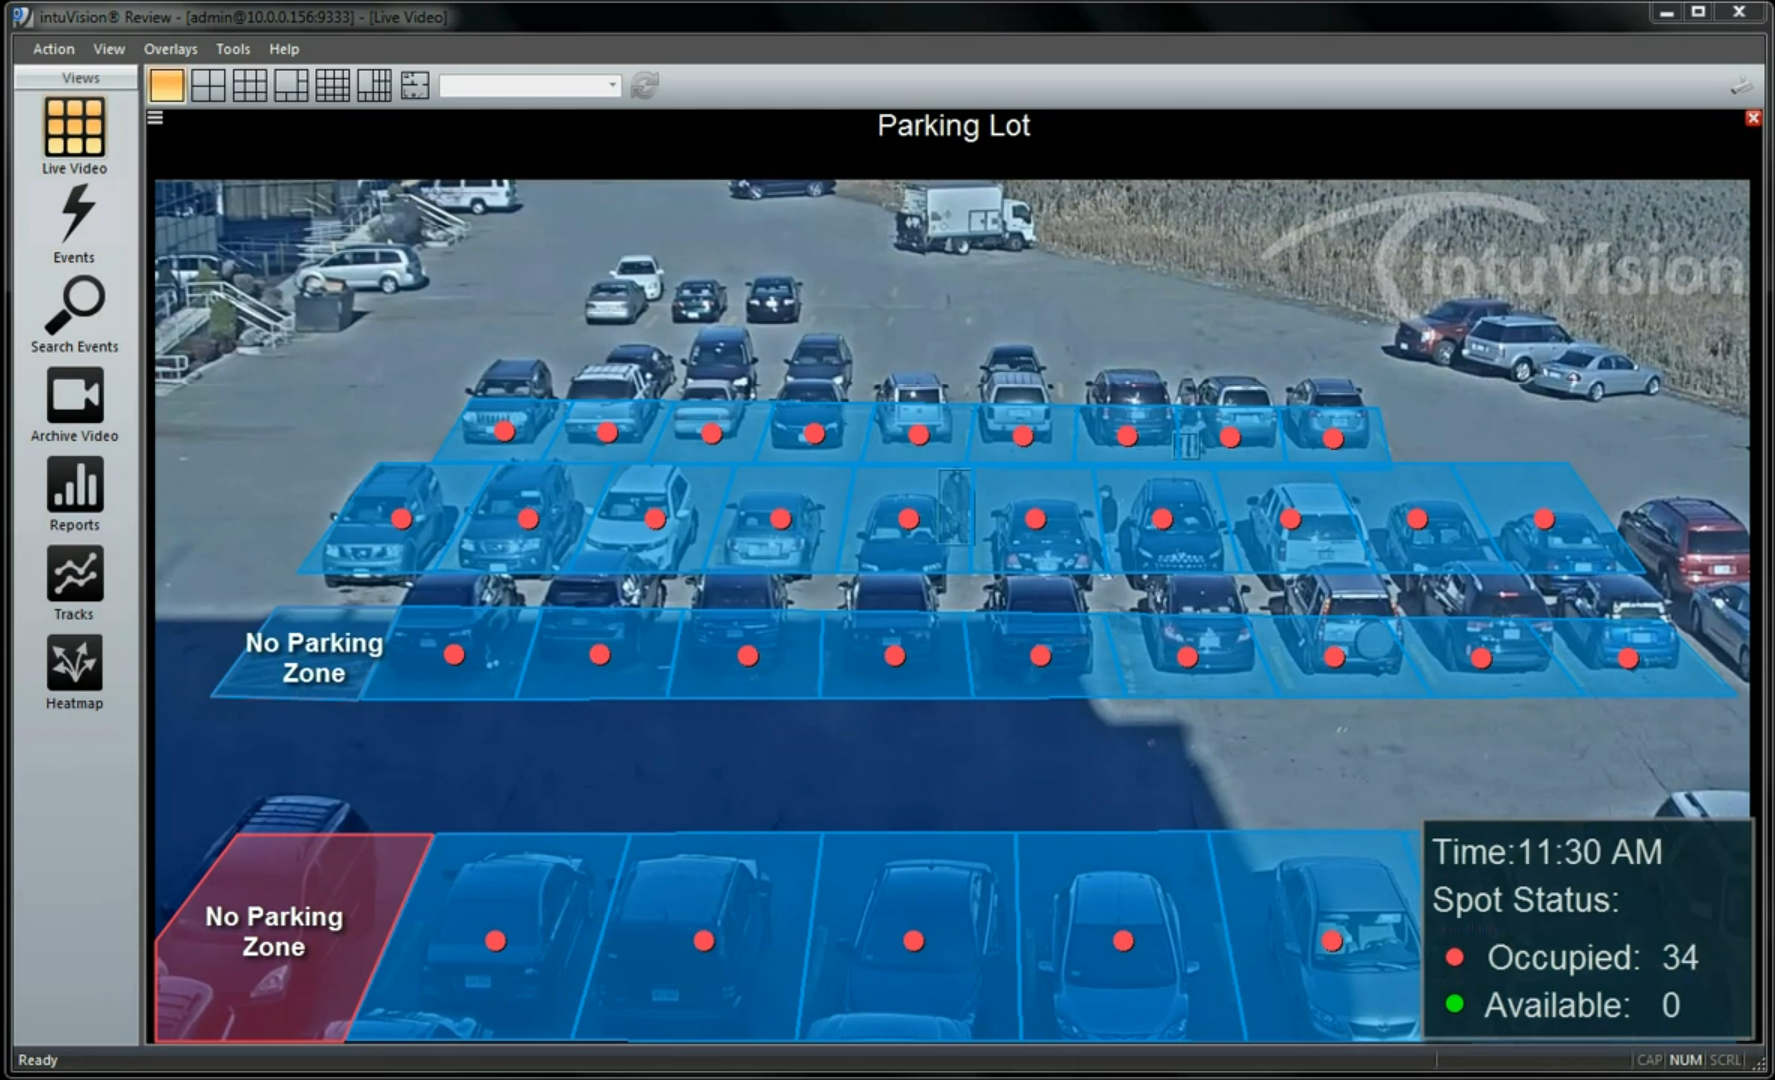
\includegraphics[width=0.8\textwidth]{/02market_research/intuvision}
	\caption{intuVision Parking Lot Demonstration.}
	\label{fig:intuvision}
\end{figure}

\section{Why choose our product}
This product aims to decrease power consumption associated with the traditional street light network, and also, using that infrastructure, contribute to the development of a smart city, detecting available parking spaces in the streets. This street lighting solution can be used in residential areas, public spaces or a large outdoor parking lot, feasible of being installed in existent lamp posts, requiring minimum changes to the original infrastructure. Although in this project it is not implemented, aside the parking spaces availability detection, this product can have the ability to monitor and to process various areas of interest using the camera built in, like for example, security purposes.


% ---------- SYSTEM ----------
\chapter{System}
\section{Network Architecture}
% Network Architecture
The system to be developed is inserted in a network, more specifically, an infrastructure based network, as shown in figure \ref{fig:infr_based_arch}. This type of networks are composed by wireless segments of a more extensive network, whose core is usually a wired network. Infrastructure-based networks have a special station, called an \ac{ap} or \ac{bs}, which serves as an interface between the wireless segment and the rest of the network. Inside the wireless segment, there will be a centralized communication, so that all messages that circulate on the network pass through a central station. That way, the network only supports two transmission directions: the downward direction (downlink), from the base station to the other stations, and the uplink direction, from the stations to the base station. The downlink usually allows the simultaneous transmission of information to a group of stations in the cell (multicast) or to all stations (broadcast).

\begin{figure}[ht]
	\centering
	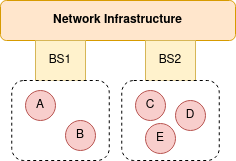
\includegraphics[width=.36\textwidth]{/03system_overview/infrastructure_based}
	\caption{Infrastructure based network architecture.}
	\label{fig:infr_based_arch}
\end{figure}

Street lighting is generally divided into sectors, facilitating maintenance and problem solving regarding the lighting network. In figure \ref{fig:network_arch}, one can see that the base station is a “special station”, since it connects the local network of lighting poles to other base stations, through a remote server, and also because it has a camera for the detection of available parking spaces. The rest of the stations that compose the local network, the local systems, will only do the smart management of their lamps.

\begin{figure}[ht]
	\centering
	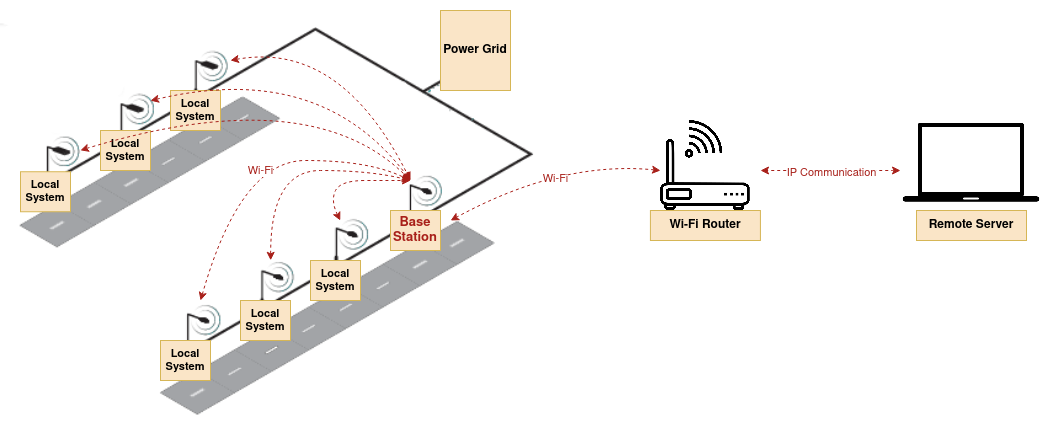
\includegraphics[width=1\textwidth]{/03system_overview/network_arch}
	\caption{Network architecture.}
	\label{fig:network_arch}
\end{figure}

The range of a Wi-Fi network depends primarily on the number and type of wireless access points used to build it, and so, the cost to build and maintain these networks increases significantly as the range increases.

The Wi-Fi signal range of any given access point also varies significantly from device to devices, depending on the specific 802.11 protocol that its used, the strength of its device transmitter and the nature of physical obstructions or radio interferences in the surrounding area. Also, due to laws of physics, 5 GHz Wi-Fi connections are more susceptible to obstructions than are 2.4 GHz. Generally, Wi-Fi routers operating on the traditional 2.4 GHz band reach up to 46 meters indoors and 92 meters outdoors. \cite{wi_fi_range}

Using a router running 802.11n, in open space the wi-fi signal range can be a little over 60 meters. \cite{wi_fi_802_11n} That being said, if each lamppost is spaced by 4 meters, each base station can easily connect with 10 local systems. To communicate with a remote server, the router will be connected to the internet through an Ethernet cable, or similar, that will most certainly already exist near the lampposts, in the telecommunications infrastructure.



% System Overview
% Requirements & Constraints
% System Architecture
\subsection{System Overview}
Through the system overview diagram, in figure \ref{fig:system_overview}, it is possible to identify the main modules of the system to be developed, and how they interact. We can divide the system into two subsystems: the local system, which represents a lamp post, and the remote system, that allows interaction with the system users.

\begin{figure}[ht]
	\centering
	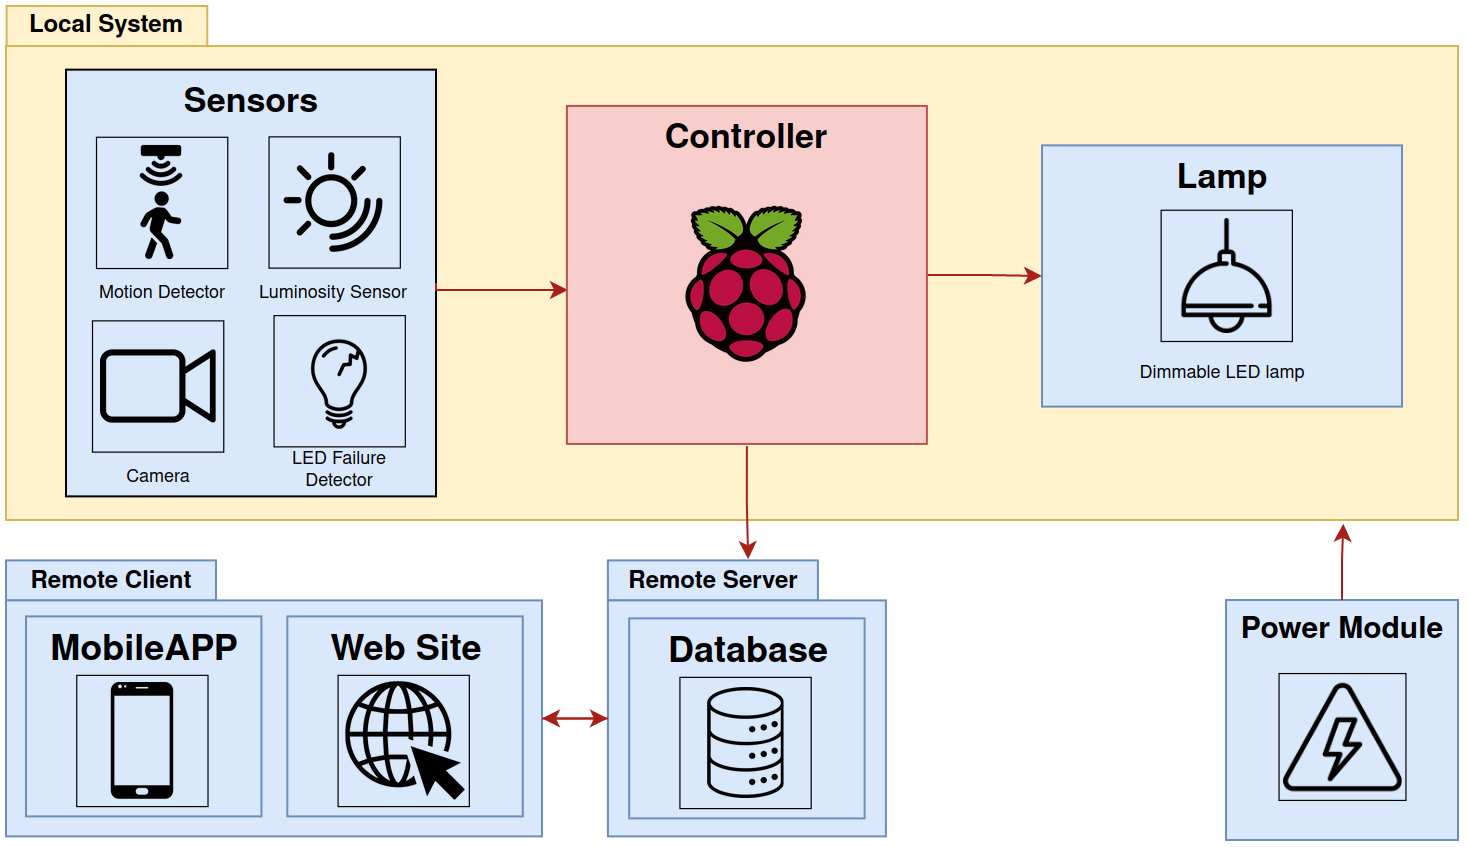
\includegraphics[width=1\textwidth]{system_overview}
	\caption{System Overview Diagram.}
	\label{fig:system_overview}
\end{figure}

The local system is composed of sensors, a controller and a lamp. Regarding the sensors, there will be a motion detector, to allow the detection of movement in the vicinity of the pole, a luminosity sensor, to detect the light conditions of the pole’s surroundings, a camera to find empty parking spots and a LED failure detector to know if the LED lamp is working. The controller, through sensors information, controls the luminosity of the lamp and communicates through the internet with a remote server, via Wi-Fi connection. 
The remote server consists of a database that stores all information about each lamp post location and operating status. This information can be accessed through a mobile application by the operator  responsible for the street lights network, in order to carry out the necessary maintenance of the lamp of each pole. Furthermore, the operator when installing a new lamp post can add its location to the database, using the mobile application. In addition, the database stores information on available parking spaces. When a user, a car driver, wants to know where there are empty parking places, he can access a website that informs him of the location of the empty parking spaces. \textbf{Knowing that the public lighting network is directly related to the electrical network, this will be used to power the local systems.}

\subsection{System Requirements and Constraints}
In order for the system to have the desired performance, these requirements and constraints must be respected:

\subparagraph{Functional Requirements}
\begin{itemize}
	\item Sensors data acquisition				
	\item Motion detector
	\item Control of a street lamp
	\item Wi-Fi communication
	\item Empty parking spots detection
	\item Manage system information through a mobile application
	\item Add lamp post location through a mobile application
	\item Access available parking spots location through a web site
\end{itemize}

\subparagraph{Non-Functional Requirements}
\begin{itemize}
	\item User friendly mobile application and web site
	\item Ambient luminosity sensing
	\item Lower power consumption than actual street lights
	\item Soft Real-Time Embedded System
\end{itemize}

\subparagraph{Technical Constraints}
\begin{itemize}
	\item Buildroot
	\item C and C++ 
	\item Device Drivers
	\item Linux
	\item Raspberry Pi
	\item \ac{cps}
	\item Makefiles
	\item Pthreads
\end{itemize}

\subparagraph{Non-Technical Constraints}
\begin{itemize}
	\item Two members team
	\item Project deadline at the end of the semester
	\item Low budget
\end{itemize}

\section{System Architecture}
Using the system overview diagram information, one can describe the system in two different architectures. Hardware architecture, as how the hardware modules interfaces with itself, and what are the physical components of the system, and software architecture, which details how the information is processed among different software layers.

\subsection{Hardware Architecture}
In figure \ref{fig:hw_arch}, one can see the diagram that represents the physical connections of the system. The power of most system components will be the output of the DC/DC converter, powering the controller and its associated sensors. In order to power the lamp and at the same time control its brightness, a driver must be used, taking the controller output and system power as inputs. The Raspberry Pi, despite not belonging to the local system, is powered similarly to the controller, via a DC/DC converter. Furthermore, it communicates with the controller wirelessly through its wireless interface, with the controller's wireless communication module.

\begin{figure}[ht]
	\centering
	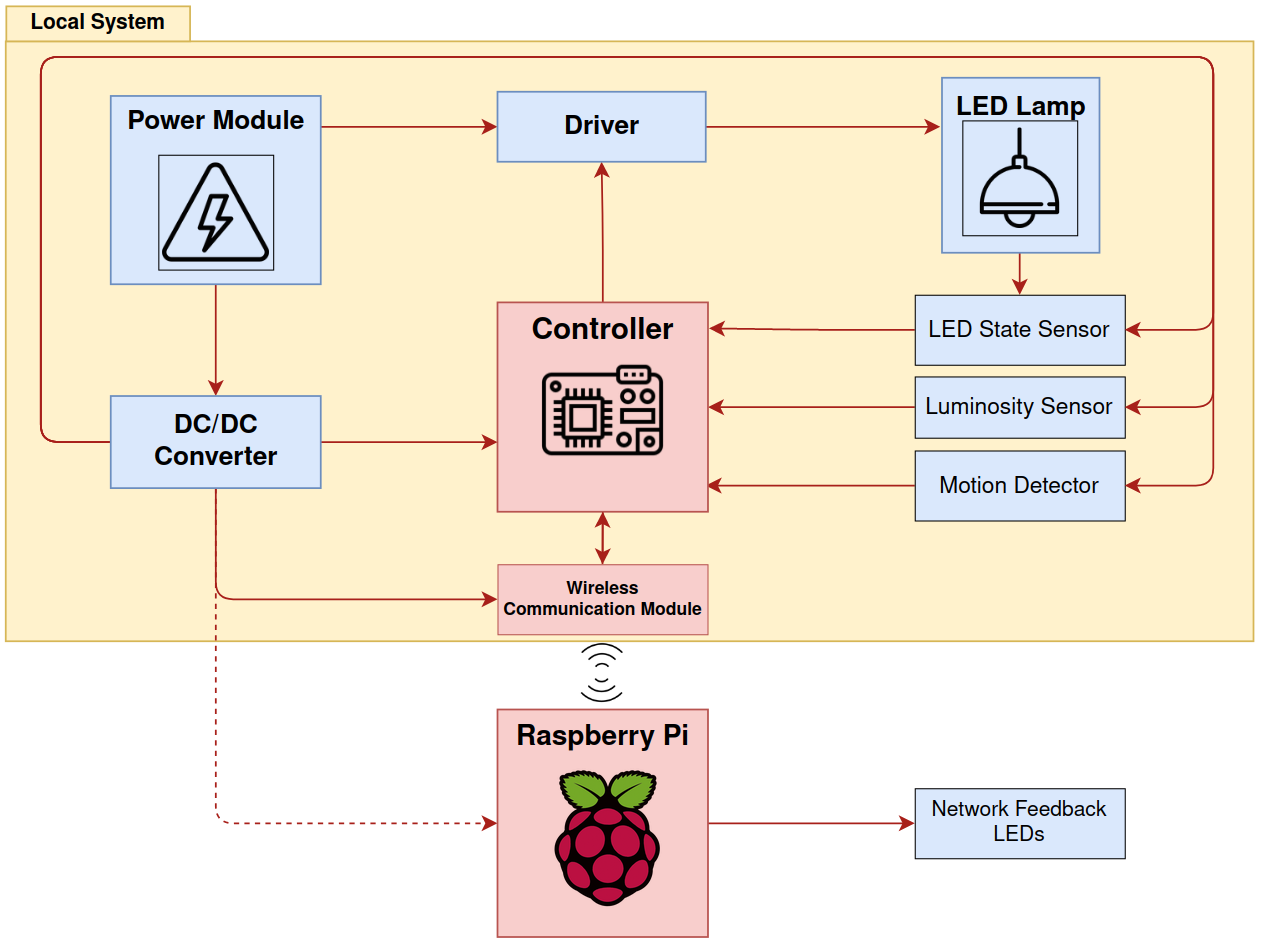
\includegraphics[width=1\textwidth]{hw_arch}
	\caption{Hardware Architecture Diagram.}
	\label{fig:hw_arch}
\end{figure}

\subsection{Software Architecture}
As seen previously, the system is divided into two subsystems: the local system and the monitoring system. Their software architectures are divided into three layers:

\begin{itemize}
	\item The Operating System layer, which is composed by the Operating System drivers and Board Support Packages;
	\item The Middleware layer, which includes software for abstracting the lower level layer packages. It works as a pipe since it links two applications, in different layers, so that data can be easily transmitted;
	\item The Application layer, where the core functionality of the program is built, with a resource for the API's in the lower level layers.
\end{itemize}

Regarding the local system, shown in figure \ref{fig:sw_arch_local}, the operating system layer is composed by the sensor drivers, such as the LED Failure Sensor, the Luminosity Sensor, the Motion Detector Sensor and also the Wireless Communication driver. As this system will acquire data from the environment through the mentioned sensors, at a low rate, and communicate this data to the monitoring device, multitasking will not be necessary, so this system will be bare metal, that is, it won’t have an operating system. In the middleware layer are the tools needed to acquire data from sensors and communicate wirelessly with the monitoring system. Finally, the communication between the different devices is managed in the application layer.

\begin{figure}[ht]
	\centering
	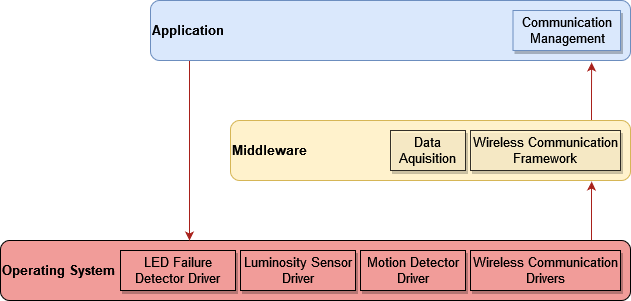
\includegraphics[width=1\textwidth]{sw_arch_local}
	\caption{Software Architecture Diagram - Local System.}
	\label{fig:sw_arch_local}
\end{figure}

Regarding the monitoring system, represented in figure \ref{fig:sw_arch_rasp}, the operating system layer is responsible for the network feedback LED drivers and for the wireless communication driver. This operating system will be a \ac{rtos}, due to the need to respond to events in a certain period of time and also multitasking. In the middleware layer, there will be the PThreads execution model, for multitasking, as well as the wireless communication and data acquisition frameworks. The application layer manages the system database, as well as the graphical user interface and all communications with local systems.

\begin{figure}[ht]
	\centering
	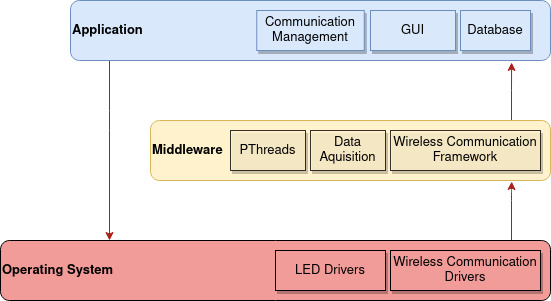
\includegraphics[width=1\textwidth]{sw_arch_rasp}
	\caption{Software Architecture Diagram - Monitoring System.}
	\label{fig:sw_arch_rasp}
\end{figure}


% ---------- SYSTEM ANALYSIS ----------
\chapter{System Analysis}

\section{Base Station}
\subsection{Events}

\begin{table}[h]
	\centering
	\resizebox{\columnwidth}{!}{
	\begin{tabular}{||c | c | c | c||} 
		\hline
		\textbf{Event} & \textbf{System Response} & \textbf{Source} & \textbf{Type}\\
		\hline\hline
Luminosity detector OFF & Power the lamp & Environment & Asynchronous\\\hline
LED failure detector ON & Notify remote system & Local system & Asynchronous\\\hline
Motion detected & Turn on the lamp & User & Asynchronous\\\hline
Requested to turn on the lamp & Turn on the lamp & Local system & Asynchronous\\\hline
Camera sample & Image processing & Timer & Synchronous\\\hline
Update system information & Send data to remote system & Local system & Asynchronous\\
		\hline
	\end{tabular}
	}		
	
	\caption{Base station events.}
	\label{table:data}
\end{table}


\subsection{Use Cases}

\begin{figure}[ht]
	\centering
	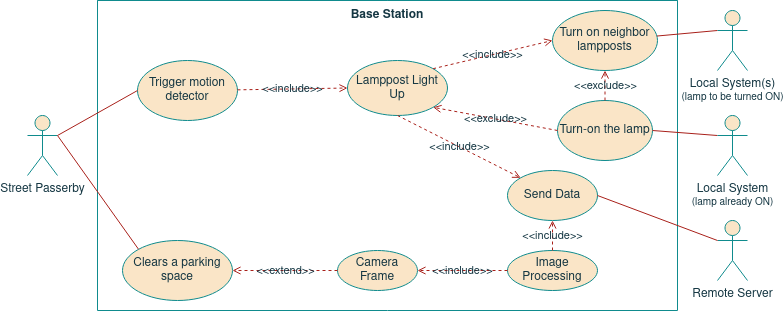
\includegraphics[width=.85\textwidth]{/05base_station/BS_UseCase}
	\caption{Base station use cases.}
	\label{fig:bs_use_cases}
\end{figure}

\subsection{State Chart}

\begin{figure}[ht]
	\centering
	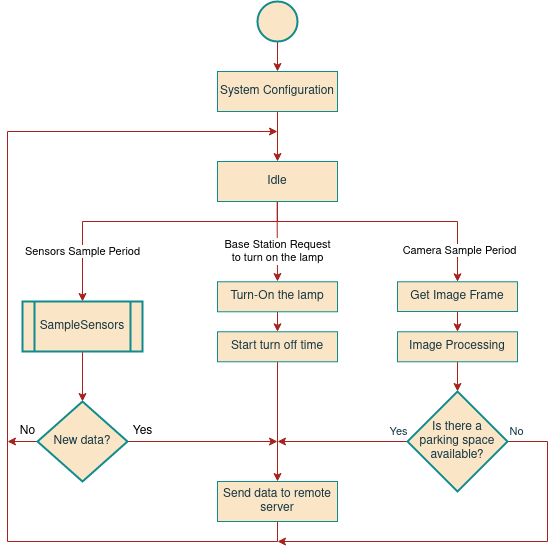
\includegraphics[width=.85\textwidth]{/05base_station/BS_StateChart}
	\caption{Base station state chart.}
	\label{fig:bs_state_chart}
\end{figure}

\begin{figure}[ht]
	\centering
	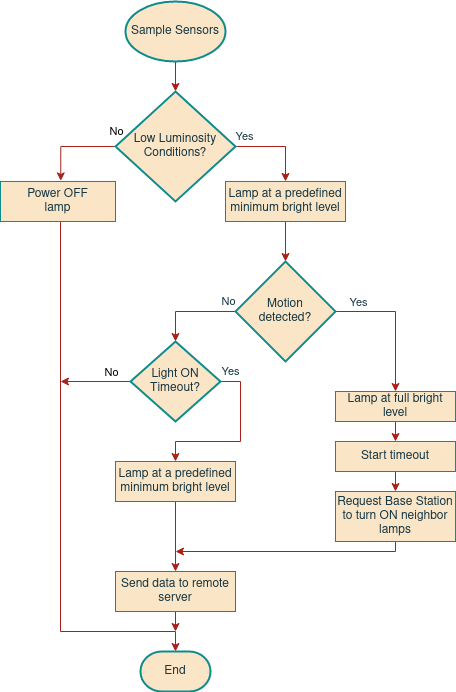
\includegraphics[width=.85\textwidth]{/05base_station/SampleSensors}
	\caption{Sampling of the sensors state chart.}
	\label{fig:sample_sensors}
\end{figure}

\subsection{Sequence Diagram}

\begin{figure}[ht]
	\centering
	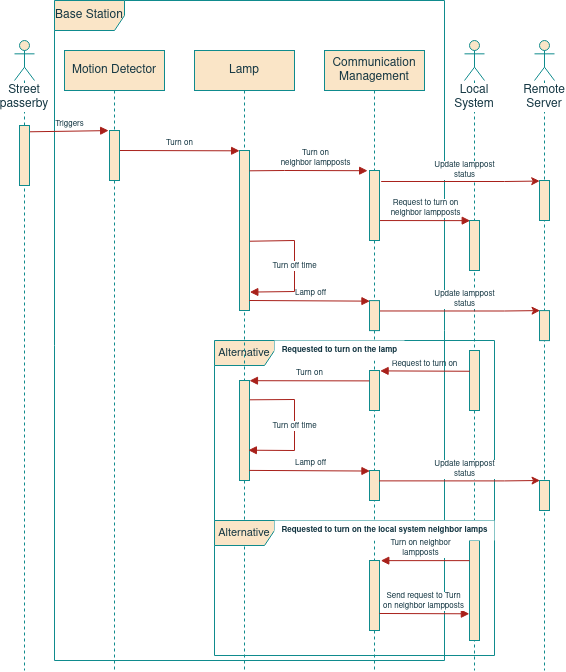
\includegraphics[width=.85\textwidth]{/05base_station/BS_SeqDiagram}
	\caption{Base station sequence diagram.}
	\label{fig:bs_seq_diagram}
\end{figure}

\section{Local System}
The local system's analysis is very similar to the base station analysis. Comparing to the base station, this system doesn't implement the parking spaces detection, since it doesn't have a camera, and only communicates with the base station. As in the base station, one can say that this is a passive system since it is most of the time waiting for something to happen.

\subsection{Events}
Listed in the table below, table \ref{table:ls_events}, are the main events that will occur in the local system and will affect its behavior. 

\begin{table}[h]
	\centering
	\resizebox{\columnwidth}{!}{
	\begin{tabular}{||c | c | c | c||} 
		\hline
		\textbf{Event} & \textbf{System Response} & \textbf{Source} & \textbf{Type}\\
		\hline\hline
Luminosity detector OFF & Power the lamp & Environment & Asynchronous\\\hline
LED failure detector ON & Notify remote system & Local system & Asynchronous\\\hline
Motion detected & Turn on the lamp & User & Asynchronous\\\hline
Requested to turn on the lamp & Turn on the lamp & Base station & Asynchronous\\\hline
Sensors data acquisition & Sample sensor values & Timer & Synchronous\\\hline
Update system information & Send data to remote system & Base station & Asynchronous\\
		\hline
	\end{tabular}
	}		
	
	\caption{Local system events.}
	\label{table:ls_events}
\end{table}

\subsection{Use Cases}
The local system use cases are represented on figure \ref{fig:ls_use_cases}. Like the base station, a street passerby, can interact with the local system by moving in the vicinity of the lamppost, triggering it's motion detector.

When movement is detected, the lamp is turned on and requests the base station to turn on the local system's neighbor lampposts. At the same time, the information that the lamppost was activated is sent to the base station, for this to be sent to the remote system.

Also, the local system can be asked, by the base station, to turn on its lamp.
\clearpage

\begin{figure}[ht]
	\centering
	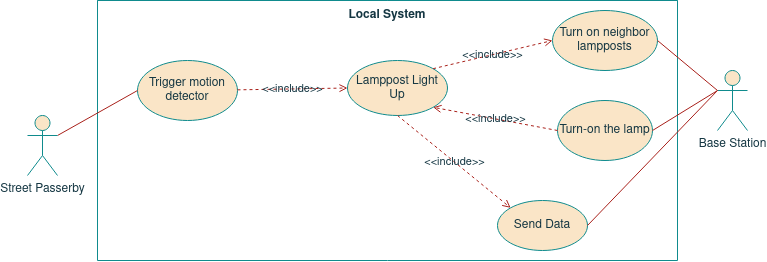
\includegraphics[width=1\textwidth]{/04local_system/LS_UseCase}
	\caption{Local system use cases.}
	\label{fig:ls_use_cases}
\end{figure}

\subsection{State Chart}
In figure \ref{fig:ls_state_chart} is represented the state chart of the local system. After the system configuration, which initializes the Wi-Fi communication management, sensors data acquisition, the system enters an idle state. To do the sensors data acquisition, like in the base station, it is used a sample period, that periodically triggers the execution of the function “SampleSensors”, presented previously, in figure \ref{fig:sample_sensors}. When the local system is requested by the base station to turn on its lamp, the lamp is turned-on and a timeout is started (turn off time, as mentioned before). The lamppost status is then sent to the base station, in order to send it to the remote server.

\begin{figure}[ht]
	\centering
	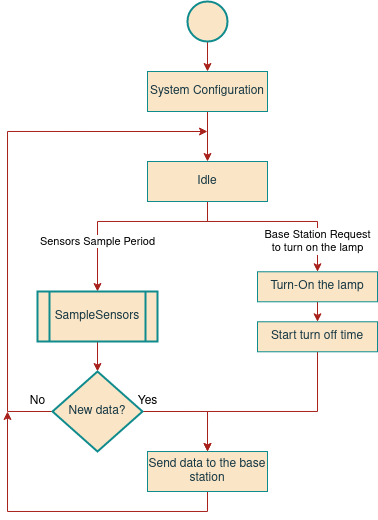
\includegraphics[width=.60\textwidth]{/04local_system/LS_StateChart}
	\caption{Local system state chart.}
	\label{fig:ls_state_chart}
\end{figure}

\clearpage
\subsection{Sequence Diagram}
The sequence diagram for the local system is represented in figure \ref{fig:ls_seq_diagram}. Again, this diagram is analogous to the one shown on the base station (figure \ref{fig:bs_seq_diagram}), having the differences that the local system only communicates with the base station, so any request that the local system wants to make to another local system has to go through the base station, and, due to that, the local system doesn't have the power to request another local system to turn its lamp on.

\begin{figure}[ht]
	\centering
	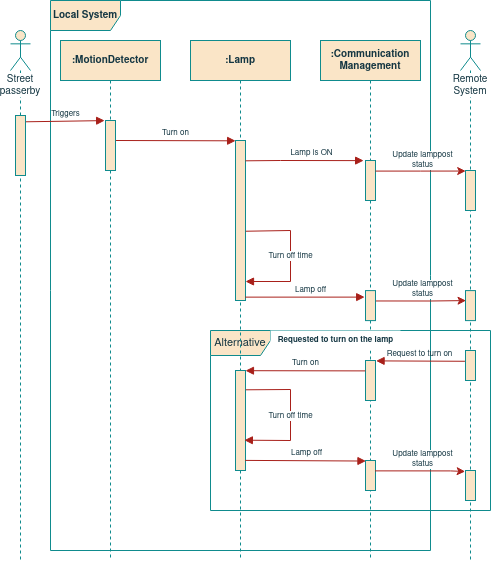
\includegraphics[width=.95\textwidth]{/04local_system/LS_SeqDiagram}
	\caption{Local system sequence diagram.}
	\label{fig:ls_seq_diagram}
\end{figure}

\section{Remote System}
\subsection{Events}

\begin{table}[ht]
	\centering
	\resizebox{\columnwidth}{!}{
	\begin{tabular}{||c | c | c | c||} 
		\hline
		Event & System Response & Source & Type\\
		\hline\hline
Login & Show application main screen if successful & Operator & Asynchronous\\\hline
Obtain geolocation & Request device geolocation & Mobile device & Asynchronous\\\hline
App notification & Notifies the operator about the lamppost status & Remote Server & Asynchronous\\\hline
Register operator & Add operator information to databas & Operator & Asynchronous\\\hline
Modify lamppost & Update lamppost information to database & Operator & Asynchronous\\\hline
Register lamppost & Add lamppost information to database & Operator & Asynchronous\\\hline
Insert location	& Show parking spots & User & Asynchronous\\\hline
Obtain geolocation & Request device geolocation & Mobile Device & Asynchronous
		\\\hline
	\end{tabular}
	}
		
	\caption{Remote system events.}
	\label{table:data}
\end{table}


\subsection{Use Cases}

\subsection{State Chart}

\subsection{Sequence Diagram}

\section{Estimated Budget}
\begin{table}[ht]
	\centering
	
	\begin{tabular}{||c | c||} 
		\hline
		\textbf{Product} & \textbf{Price(€)}\\
		\hline\hline
		Raspberry Pi 4B & 63,50\\\hline
		Industrial power supply 12 V & 5,00\\\hline
		Video camera & 8,86\\\hline
		Motion detector & 4,60\\\hline
		Luminosity sensor & 1,69\\\hline
		LED lamp 12 V & 3,63\\\hline
		Driver (MOSFET) & 1,00\\\hline
		Basic Eletronic Components & 5,00\\\hline
		\hline
		\textbf{Total} & \textbf{93,28}\\\hline
	\end{tabular}
	\caption{Estimated budget.}
	\label{table:data}
\end{table}

% Task Division and Gantt Chart
% Task Division/Gantt
\section{Task Division and Gantt Chart}
In figure x, is represented the Smart Street Lighting project schedule in form of a Gantt chart.

\begin{figure}[ht]
	\centering
	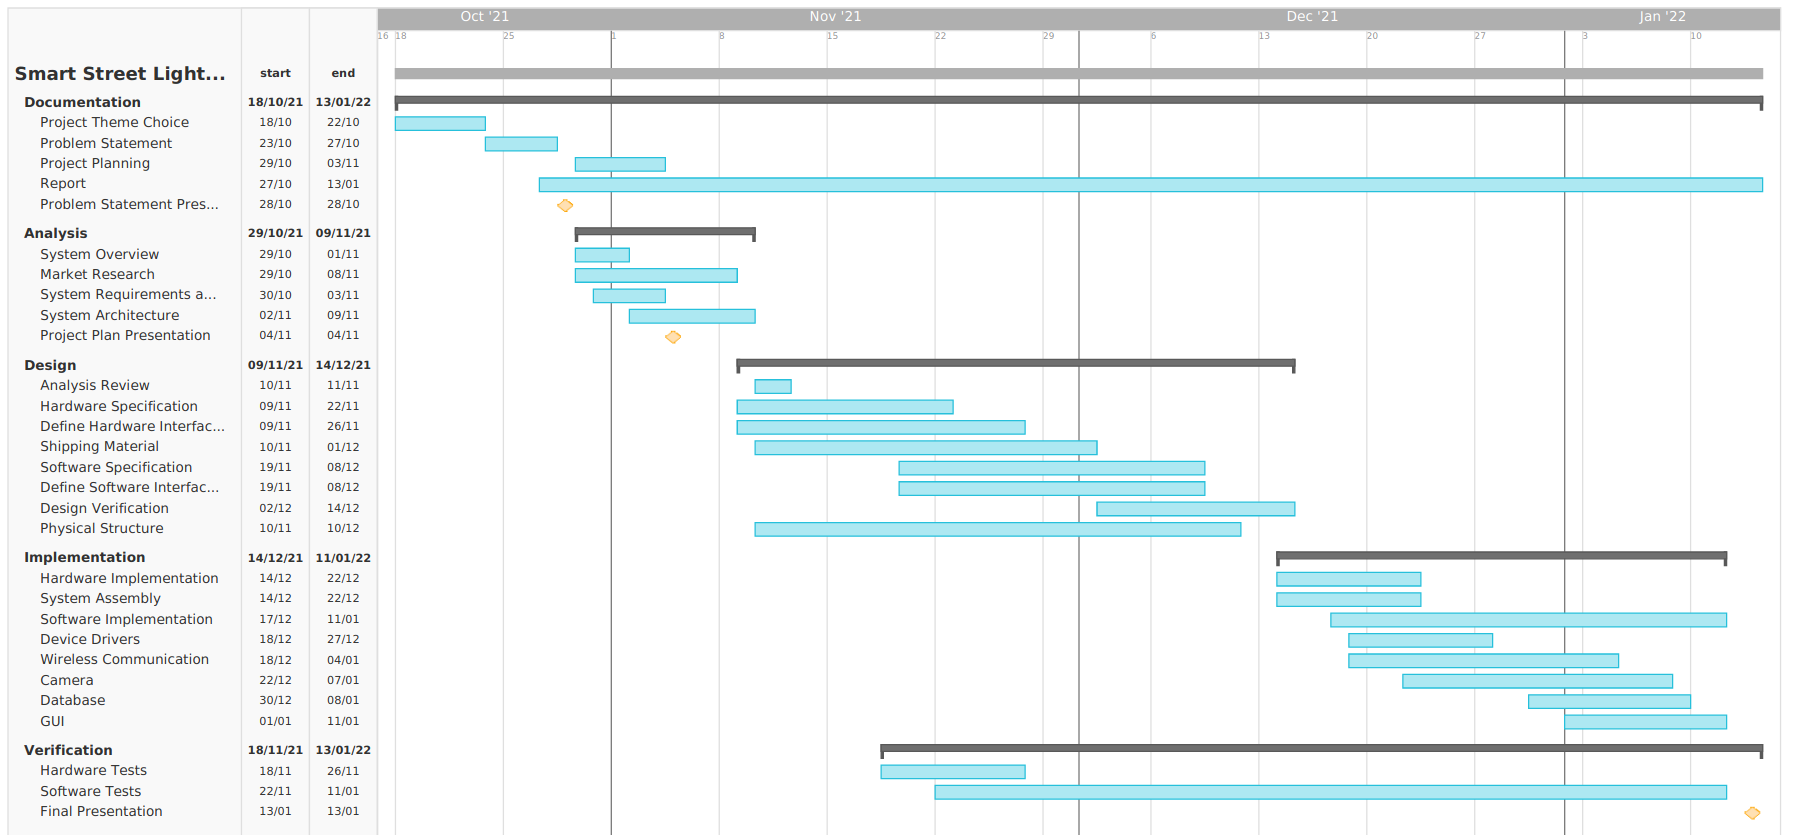
\includegraphics[width=1\textwidth]{Gantt_chart}
	\caption{Gantt chart.}
	\label{fig:Gantt_chart}
\end{figure}



% ---------- BIBLIOGRAPHY ----------
\bibliographystyle{IEEEtran}
\bibliography{References}

\end{document}